\section{Reversible FFT}
As mentioned in section \ref{sec:fourier},
both FT and DFT are invertible sums.
The definition of IDFT also permits a factorization that is essentially equivalent to that of the DFT.
However, we wish to write a reversible DFT that can be directly inverted to obtain an IDFT.
There are some challenges that must be overcome in order to do this.
Most of the challenges are detailed in \cite{intfft}, which also presents solutions to these.

\subsection{In-place computation}
The FFT algorithm described in the previous section
creates two new arrays of even- and odd-indexed elements.
Rather than create new arrays,
we can rearrange the evens and odds into the upper and lower half of the array,
then recurse on these halfs.
This allows the transform to be performed in-place.

Taking it further, rather than rearranging the array at every recursion step,
we can perform a single equivalent rearrangement of the array at the start of the algorithm.
This is usually referred to as a scrambling of the array.
In order to get an arrangement equivalent to recursively separating evens and odds down to the base case,
we swap the element at each index with the index obtained from reversing its bit string.

After scrambling,
we have $N/2$ pairs of even and odd base cases placed next to each other.
These can be merged, giving us $N/4$ pairs of size 2 FFT solutions.
We then merge these solutions into $N/8$ size 4 solutions,
and repeat until we have obtained an FFT for the full array.
Figure \ref{fig:lattice} shows this strategy in action for an array of size 8.
\begin{figure}
    \centering
    \resizebox{\textwidth}{!}{%
    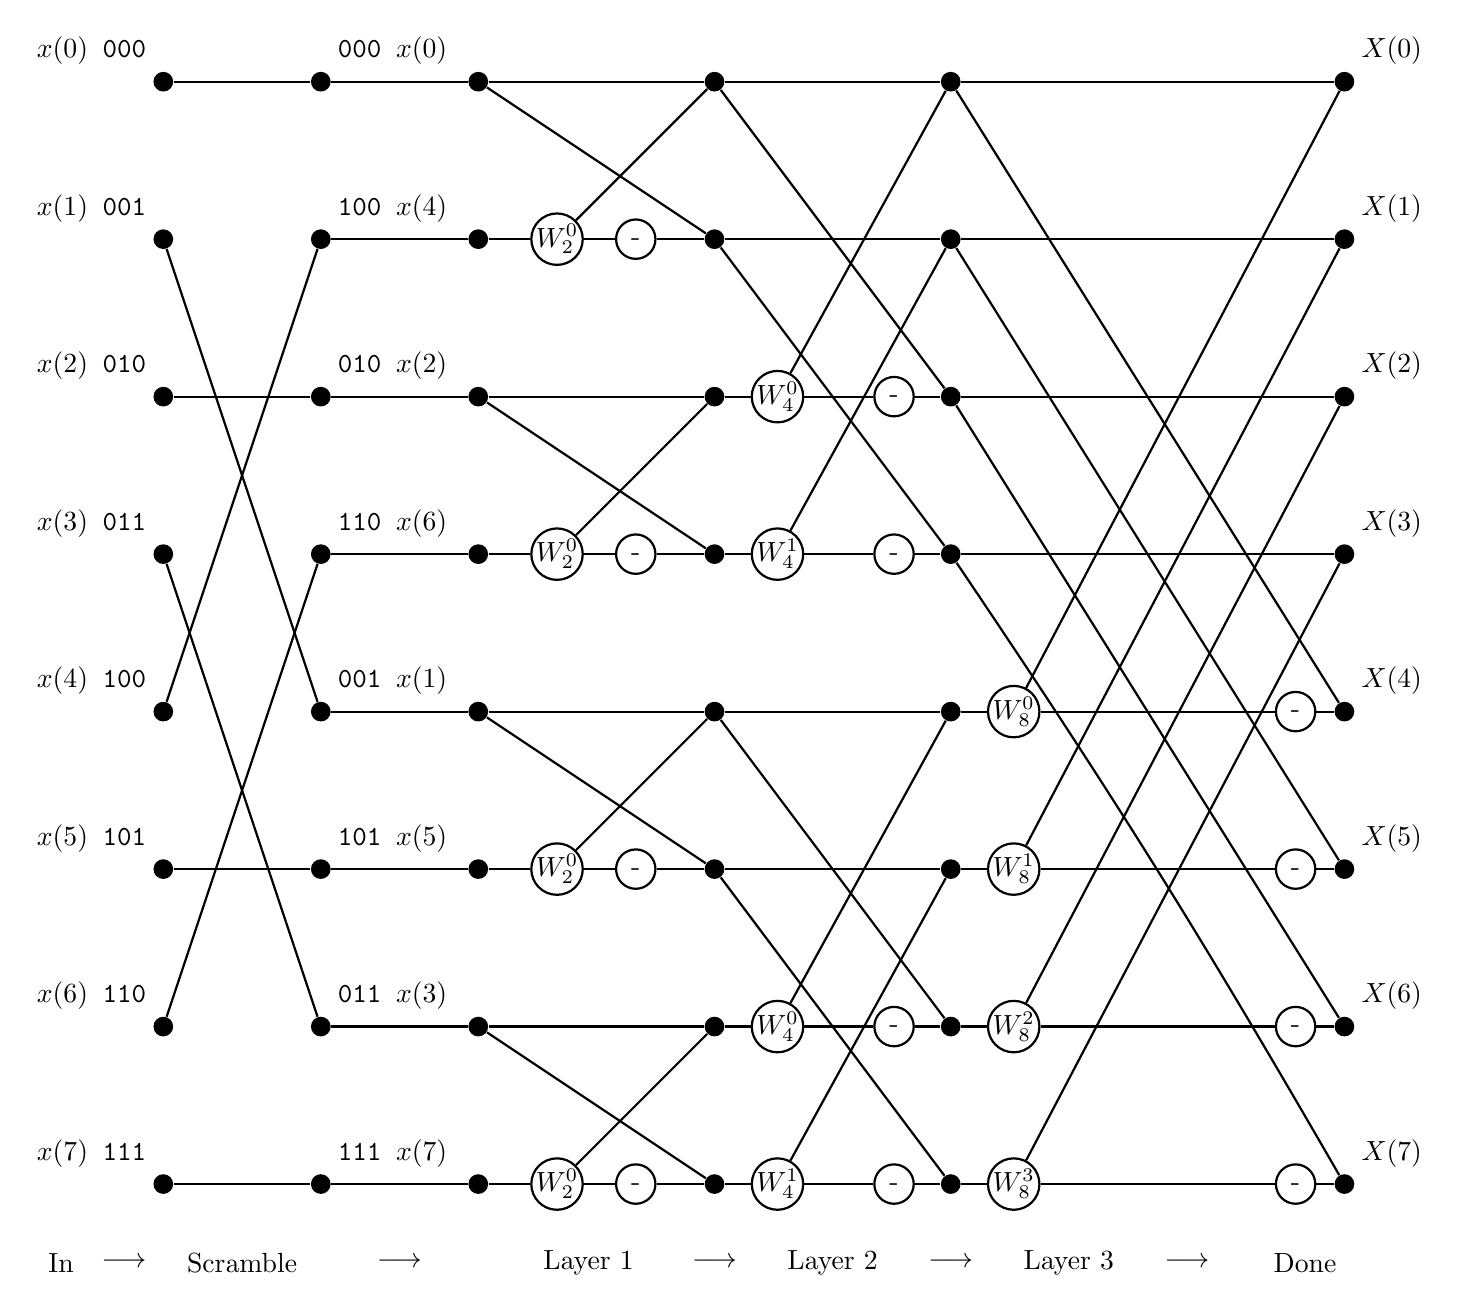
\begin{tikzpicture}[
        dot/.style = {circle, fill, inner sep = 0mm, minimum size = 2.5mm},
        op/.style = {draw, thick, circle, inner sep = 0mm, minimum size = 5mm},
        func/.style = {draw, thick, circle, inner sep = 1mm},
        arr/.style = {draw, thick},
    ]
        \node (in0) at (0, 14) [dot, label=above left:$x(0)$\texttt{ 000}]{};
        \node (in1) at (0, 12) [dot, label=above left:$x(1)$\texttt{ 001}]{};
        \node (in2) at (0, 10) [dot, label=above left:$x(2)$\texttt{ 010}]{};
        \node (in3) at (0,  8) [dot, label=above left:$x(3)$\texttt{ 011}]{};
        \node (in4) at (0,  6) [dot, label=above left:$x(4)$\texttt{ 100}]{};
        \node (in5) at (0,  4) [dot, label=above left:$x(5)$\texttt{ 101}]{};
        \node (in6) at (0,  2) [dot, label=above left:$x(6)$\texttt{ 110}]{};
        \node (in7) at (0,  0) [dot, label=above left:$x(7)$\texttt{ 111}]{};

        \node (sc0) at (2, 14) [dot, label=above right:\texttt{000 }$x(0)$]{};
        \node (sc4) at (2, 12) [dot, label=above right:\texttt{100 }$x(4)$]{};
        \node (sc2) at (2, 10) [dot, label=above right:\texttt{010 }$x(2)$]{};
        \node (sc6) at (2,  8) [dot, label=above right:\texttt{110 }$x(6)$]{};
        \node (sc1) at (2,  6) [dot, label=above right:\texttt{001 }$x(1)$]{};
        \node (sc5) at (2,  4) [dot, label=above right:\texttt{101 }$x(5)$]{};
        \node (sc3) at (2,  2) [dot, label=above right:\texttt{011 }$x(3)$]{};
        \node (sc7) at (2,  0) [dot, label=above right:\texttt{111 }$x(7)$]{};

        \path[arr] (in0) -- (sc0);
        \path[arr] (in1) -- (sc1);
        \path[arr] (in2) -- (sc2);
        \path[arr] (in3) -- (sc3);
        \path[arr] (in4) -- (sc4);
        \path[arr] (in5) -- (sc5);
        \path[arr] (in6) -- (sc6);
        \path[arr] (in7) -- (sc7);

        \node (l00) at (4, 14) [dot]{};
        \node (l01) at (4, 12) [dot]{};
        \node (l02) at (4, 10) [dot]{};
        \node (l03) at (4,  8) [dot]{};
        \node (l04) at (4,  6) [dot]{};
        \node (l05) at (4,  4) [dot]{};
        \node (l06) at (4,  2) [dot]{};
        \node (l07) at (4,  0) [dot]{};

        \path[arr] (sc0) -- (l00);
        \path[arr] (sc4) -- (l01);
        \path[arr] (sc2) -- (l02);
        \path[arr] (sc6) -- (l03);
        \path[arr] (sc1) -- (l04);
        \path[arr] (sc5) -- (l05);
        \path[arr] (sc3) -- (l06);
        \path[arr] (sc7) -- (l07);

        \node (w01) at (5, 12) [op]{$W_2^0$};
        \node (w03) at (5,  8) [op]{$W_2^0$};
        \node (w05) at (5,  4) [op]{$W_2^0$};
        \node (w07) at (5,  0) [op]{$W_2^0$};

        \node (m01) at (6, 12) [op]{-};
        \node (m03) at (6,  8) [op]{-};
        \node (m05) at (6,  4) [op]{-};
        \node (m07) at (6,  0) [op]{-};

        \node (l10) at (7, 14) [dot]{};
        \node (l11) at (7, 12) [dot]{};
        \node (l12) at (7, 10) [dot]{};
        \node (l13) at (7,  8) [dot]{};
        \node (l14) at (7,  6) [dot]{};
        \node (l15) at (7,  4) [dot]{};
        \node (l16) at (7,  2) [dot]{};
        \node (l17) at (7,  0) [dot]{};

        \path[arr] (l01) -- (w01);
        \path[arr] (l03) -- (w03);
        \path[arr] (l05) -- (w05);
        \path[arr] (l07) -- (w07);
        \path[arr] (w01) -- (m01);
        \path[arr] (w03) -- (m03);
        \path[arr] (w05) -- (m05);
        \path[arr] (w07) -- (m07);
        \path[arr] (m01) -- (l11);
        \path[arr] (m03) -- (l13);
        \path[arr] (m05) -- (l15);
        \path[arr] (m07) -- (l17);

        \path[arr] (w01) -- (l10);
        \path[arr] (w03) -- (l12);
        \path[arr] (w05) -- (l14);
        \path[arr] (w07) -- (l16);
        \path[arr] (l00) -- (l10);
        \path[arr] (l02) -- (l12);
        \path[arr] (l04) -- (l14);
        \path[arr] (l06) -- (l16);
        \path[arr] (l00) -- (l11);
        \path[arr] (l02) -- (l13);
        \path[arr] (l04) -- (l15);
        \path[arr] (l06) -- (l17);

        \node (w12) at (7.8, 10) [op]{$W_4^0$};
        \node (w13) at (7.8,  8) [op]{$W_4^1$};
        \node (w16) at (7.8,  2) [op]{$W_4^0$};
        \node (w17) at (7.8,  0) [op]{$W_4^1$};

        \node (m12) at (9.28, 10) [op]{-};
        \node (m13) at (9.28,  8) [op]{-};
        \node (m16) at (9.28,  2) [op]{-};
        \node (m17) at (9.28,  0) [op]{-};

        \node (l20) at (10, 14) [dot]{};
        \node (l21) at (10, 12) [dot]{};
        \node (l22) at (10, 10) [dot]{};
        \node (l23) at (10,  8) [dot]{};
        \node (l24) at (10,  6) [dot]{};
        \node (l25) at (10,  4) [dot]{};
        \node (l26) at (10,  2) [dot]{};
        \node (l27) at (10,  0) [dot]{};

        \path[arr] (l10) -- (l20);
        \path[arr] (l10) -- (l22);
        \path[arr] (l11) -- (l21);
        \path[arr] (l11) -- (l23);
        \path[arr] (l14) -- (l24);
        \path[arr] (l14) -- (l26);
        \path[arr] (l15) -- (l25);
        \path[arr] (l15) -- (l27);

        \path[arr] (w12) -- (l20);
        \path[arr] (w13) -- (l21);
        \path[arr] (w16) -- (l24);
        \path[arr] (w17) -- (l25);

        \path[arr] (l12) -- (w12);
        \path[arr] (l13) -- (w13);
        \path[arr] (l16) -- (w16);
        \path[arr] (l17) -- (w17);

        \path[arr] (w12) -- (m12);
        \path[arr] (w13) -- (m13);
        \path[arr] (w16) -- (m16);
        \path[arr] (w17) -- (m17);

        \path[arr] (m12) -- (l22);
        \path[arr] (m13) -- (l23);
        \path[arr] (m16) -- (l26);
        \path[arr] (m17) -- (l27);

        \node (l30) at (15, 14) [dot, label=above right:$X(0)$]{};
        \node (l31) at (15, 12) [dot, label=above right:$X(1)$]{};
        \node (l32) at (15, 10) [dot, label=above right:$X(2)$]{};
        \node (l33) at (15,  8) [dot, label=above right:$X(3)$]{};
        \node (l34) at (15,  6) [dot, label=above right:$X(4)$]{};
        \node (l35) at (15,  4) [dot, label=above right:$X(5)$]{};
        \node (l36) at (15,  2) [dot, label=above right:$X(6)$]{};
        \node (l37) at (15,  0) [dot, label=above right:$X(7)$]{};

        \node (w24) at (10.8, 6) [op]{$W_8^0$};
        \node (w25) at (10.8, 4) [op]{$W_8^1$};
        \node (w26) at (10.8, 2) [op]{$W_8^2$};
        \node (w27) at (10.8, 0) [op]{$W_8^3$};

        \path[arr] (w24) -- (l30);
        \path[arr] (w25) -- (l31);
        \path[arr] (w26) -- (l32);
        \path[arr] (w27) -- (l33);

        \node (m24) at (14.38, 6) [op, fill=white]{-};
        \node (m25) at (14.38, 4) [op, fill=white]{-};
        \node (m26) at (14.38, 2) [op, fill=white]{-};
        \node (m27) at (14.38, 0) [op, fill=white]{-};

        \path[arr] (l24) -- (w24);
        \path[arr] (w24) -- (m24);
        \path[arr] (m24) -- (l34);
        \path[arr] (l25) -- (w25);
        \path[arr] (w25) -- (m25);
        \path[arr] (m25) -- (l35);
        \path[arr] (l26) -- (w26);
        \path[arr] (w26) -- (m26);
        \path[arr] (m26) -- (l36);
        \path[arr] (l27) -- (w27);
        \path[arr] (w27) -- (m27);
        \path[arr] (m27) -- (l37);

        \path[arr] (l20) -> (l30);
        \path[arr] (l21) -> (l31);
        \path[arr] (l22) -> (l32);
        \path[arr] (l23) -> (l33);
        \path[arr] (l20) -> (l34);
        \path[arr] (l21) -> (l35);
        \path[arr] (l22) -> (l36);
        \path[arr] (l23) to[bend left=2] (l37);

        \node at (-1.3, -1) {In};
        \node at (-0.5, -1) {$\longrightarrow$};
        \node at (1, -1) {Scramble};
        \node at (3, -1) {$\longrightarrow$};
        \node at (5.4, -1) {Layer 1};
        \node at (7, -1) {$\longrightarrow$};
        \node at (8.5, -1) {Layer 2};
        \node at (10, -1) {$\longrightarrow$};
        \node at (11.5, -1) {Layer 3};
        \node at (13, -1) {$\longrightarrow$};
        \node at (14.5, -1) {Done};
    \end{tikzpicture}
    }%
    \caption{Example datapath representation of our FFT algorithm with $N = 8$.
    \label{fig:lattice}}
\end{figure}


\subsection{Fixpoint arithmetic}
The next problem is that we must find a way to represent complex numbers.
Complex numbers can represented by two reals $a_r, a_i \in \mathbb{R}$ such that $a = a_r + ib_i$.
Your first idea might be to use floating point numbers to represent $a_r$ and $b_i$,
but updates to floats are inherently destructive.

Instead, we use a fix-point representation.
Each real number can be written as $r = x \cdot 2^{-p},~~ x, p \in \mathbb{Z}$.
The value of $p$ is known as the fix-point for $r$,
and can be visualized as a decimal point (binary point?) in the bit string.
We will store $r$ in an integer, and $p$ will generally be implicit.
Operations on these numbers can be performed with the integer equivalents on the $x$ value.

Ignoring overflows, both addition and subtraction are invertible.
Multiplication is only injective ie. left-invertible.
This is quite clear when you consider what happens when dividing an odd number by 2.
Furthermore, it should be noted that multiplication of two numbers with fix-points $p_1$ and $p_2$
results in a number with fix-point $p_1 + p_2$.
We may wish to quantize (round) these integers to move the fixpoint back,
but this is a destructive operation.

\subsection{Lifting steps}
Some central operations of our FFT algorithm
must update two variables at once in a butterfly-like structure.
That is to say, each value must be updated in a way that is dependent on both itself and the other,
creating a datapath that looks like a ``butterfly''.
Mutually dependent simultaneous updates are a problem for reversibility,
as we cannot recover the original values.
Luckily, our specific updates \textit{can} be reversed, at least in a mathematical sense.

In order to make them practically reversible,
we can convert them into a series of \textit{lifting steps}.
This method is described in detail in \cite{lifting1998},
although we use the method for somewhat simpler tasks.

Figure \ref{fig:lift} shows the concept as datapaths.
Say we need to perform a ``butterfly'' update on two variables $A$ and $B$.
Instead of performing simultaneous updates,
we can run $B$ through some function $F$ and add it to $A$.
Next, we can run $A$ through another function $G$ and add it back to $B$.
Since the value added at each step can still be derived after the addition,
we can reverse the operation by deriving and subtracting the same values in the opposite order.

If we can represent a butterfly update as a lifting scheme, we can reverse it.
The method also has another benefit;
the in-between functions like $F$ and $G$ do not have to be reversible.
If the functions produce a lot of new information, we can quantize the result before addition.
For example, fixpoint multiplication adds some amount $p$ bits of resolution to the result,
but this can be thrown out by rounding (eg. through left-shifting) the result
before adding it to either $A$ or $B$.
\begin{figure}[h]
    \centering
    \begin{subfigure}[b]{0.45\textwidth}
        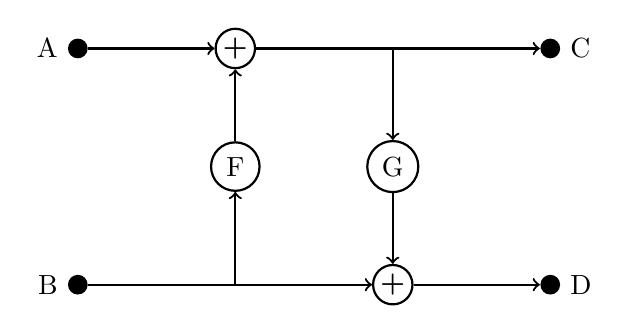
\begin{tikzpicture}[
                dot/.style = {circle, fill, inner sep = 0mm, minimum size = 2.5mm},
                op/.style = {draw, thick, circle, inner sep = 0mm, minimum size = 5mm},
                func/.style = {draw, thick, circle, inner sep = 1mm},
                arr/.style = {draw, thick, ->},
            ]
            \node (A) at (0, 3) [dot, label = left:A] {};
            \node (B) at (0, 0) [dot, label = left:B] {};
            \node (C) at (6, 3) [dot, label = right:C] {};
            \node (D) at (6, 0) [dot, label = right:D] {};

            \node (P1) at (2, 3) [op] {\textbf{+}};
            \node (P2) at (4, 0) [op] {\textbf{+}};

            \node (F) at (2, 1.5) [func] {F};
            \node (G) at (4, 1.5) [func] {G};

            \path[arr] (A) -- (P1);
            \path[arr] (P1) -- (C);
            \path[arr] (B) -- (P2);
            \path[arr] (P2) -- (D);
            \path[arr] (2, 0) -- (F);
            \path[arr] (F) -- (P1);
            \path[arr] (4, 3) -- (G);
            \path[arr] (G) -- (P2);
        \end{tikzpicture}
        \caption{Lifting steps.}
    \end{subfigure}
    \begin{subfigure}[b]{0.5\textwidth}
        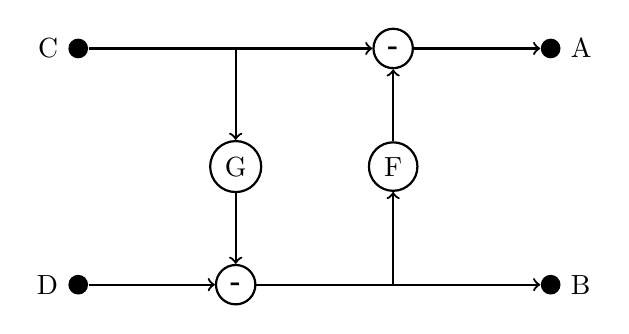
\begin{tikzpicture}[
                dot/.style = {circle, fill, inner sep = 0mm, minimum size = 2.5mm},
                op/.style = {draw, thick, circle, inner sep = 0mm, minimum size = 5mm},
                func/.style = {draw, thick, circle, inner sep = 1mm},
                arr/.style = {draw, thick, ->},
            ]
            \node (A) at (14, 3) [dot, label = right:A] {};
            \node (B) at (14, 0) [dot, label = right:B] {};
            \node (C) at (8, 3) [dot, label = left:C] {};
            \node (D) at (8, 0) [dot, label = left:D] {};

            \node (P1) at (12, 3) [op] {\textbf{-}};
            \node (P2) at (10, 0) [op] {\textbf{-}};

            \node (F) at (12, 1.5) [func] {F};
            \node (G) at (10, 1.5) [func] {G};

            \path[arr] (P1) -- (A);
            \path[arr] (C) -- (P1);
            \path[arr] (P2) -- (B);
            \path[arr] (D) -- (P2);

            \path[arr] (12, 0) -- (F);
            \path[arr] (10, 3) -- (G);
            \path[arr] (F) -- (P1);
            \path[arr] (G) -- (P2);
        \end{tikzpicture}
        \caption{Inverse path.}
    \end{subfigure}
    \caption{Dataflow path of a lifting step and its derived inverse.\label{fig:lift}}
\end{figure}


\subsection{Complex multiplication}
As a reminder, complex multiplication is performed with:
\begin{equation}
    ax = (a_r + a_i \cdot i)(x_r + x_i \cdot i) = a_rx_r - a_ix_i + (a_r x_i + a_ix_r)i
\end{equation}
If we treat complex numbers as vectors, we can represent this as a matrix multiplication:
\begin{equation}
    ax =
    \begin{bmatrix}
        a_r &-a_i\\
        a_i &a_r
    \end{bmatrix}
    \begin{bmatrix}
        x_r\\
        x_i
    \end{bmatrix}
\end{equation}
It should be clear that an in-place multiplication of $x$ with $a$ requires a simultaneous update.
Figure \ref{fig:complexmula} shows the butterfly datapath for this update.
In our case, we wish to multiply our values by a pre-known coefficient $a = W_N^k$.
We also know this value to be of unit length, meaning that $\sqrt{a_r^2 + a_i^2} = 1$.
Utilizing this equivalence, we can factorize the matrix as follows:
\begin{equation}
    ax =
    \begin{bmatrix}
        1 &\frac{c-1}{s}\\
        0 &1
    \end{bmatrix}
    \begin{bmatrix}
        1 &0\\
        s &1
    \end{bmatrix}
    \begin{bmatrix}
        1 &\frac{c - 1}{s}\\
        0 &1
    \end{bmatrix}
    \begin{bmatrix}
        x_r\\
        x_i
    \end{bmatrix}
\end{equation}
These multiplications can be performed by the lifting steps shown in figure \ref{fig:complexmulb}.
Figure \ref{fig:complexmulc} shows the lifting scheme with added quantization steps.
As for how to obtain these coefficients,
we can pre-compute them and add them to the program as a lookup table.
It is only necessary to compute the coefficients $W_N^k,~k \in (0;N/4)$, as:
\begin{itemize}
    \item $W_N^0 x$ and $W_N^{N/4} x$ can be trivially computed without coefficients.
    \item $W_N^k x$ for $k \in (N/4; N/2)$ can be computed by with $-W_N^{-k}$.
    \item $W_N^k$ for $k \in [N/2;N)$ is never used.
    \item $W_{N/2^L}^k x$ can be obtained from $W_N^{2^L k} x$.
\end{itemize}

\begin{figure}[h]
    \begin{subfigure}[b]{0.5\textwidth}
        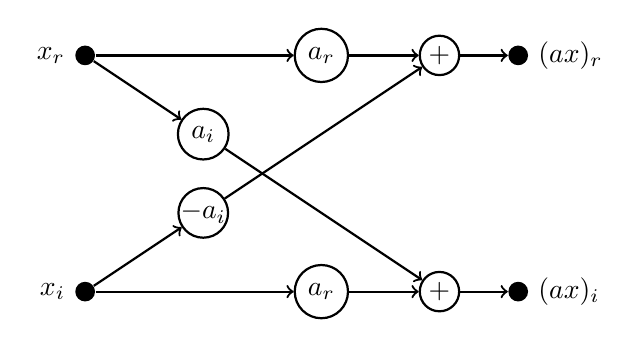
\begin{tikzpicture}[
                dot/.style = {circle, fill, inner sep = 0mm, minimum size = 2.5mm},
                op/.style = {draw, thick, circle, inner sep = 0mm, minimum size = 5mm},
                func/.style = {draw, thick, circle, inner sep = 1mm},
                arr/.style = {draw, thick, ->},
            ]
            \node (XR) [dot, label=left:$x_r$] at (0,3){};
            \node (XI) [dot, label=left:$x_i$] at (0,0){};
            \node (AXR) [dot, label=right:$(ax)_r$] at (5.5,3){};
            \node (AXI) [dot, label=right:$(ax)_i$] at (5.5,0){};

            \node (P1) [op] at (4.5, 3) {+};
            \node (P2) [op] at (4.5, 0) {+};
            \node (AR1) [func] at (3.0, 3) {$a_r$};
            \node (AR2) [func] at (3.0, 0) {$a_r$};

            \node (AI1) [func] at (1.5, 2) {$a_i$};
            \node (AI2) [op] at (1.5, 1) {$-a_i$};

            \path[arr] (XR) -- (AR1);
            \path[arr] (AR1) -- (P1);
            \path[arr] (P1) -- (AXR);

            \path[arr] (XI) -- (AR2);
            \path[arr] (AR2) -- (P2);
            \path[arr] (P2) -- (AXI);

            \path[arr] (XR) -- (AI1);
            \path[arr] (AI1) -- (P2);

            \path[arr] (XI) -- (AI2);
            \path[arr] (AI2) -- (P1);
        \end{tikzpicture}
        \caption{Butterfly structure.\label{fig:complexmula}}
    \end{subfigure}
    \begin{subfigure}[b]{0.5\textwidth}
        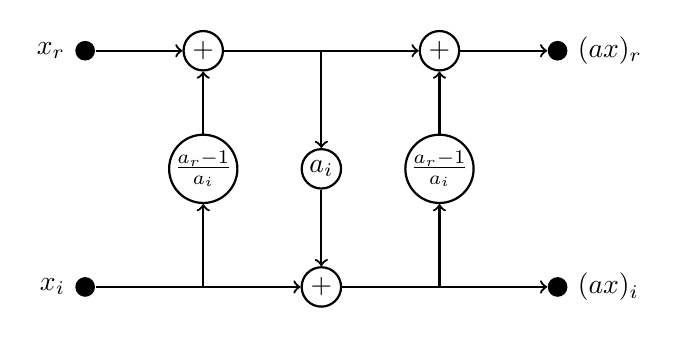
\begin{tikzpicture}[
                dot/.style = {circle, fill, inner sep = 0mm, minimum size = 2.5mm},
                op/.style = {draw, thick, circle, inner sep = 0mm, minimum size = 5mm},
                func/.style = {draw, thick, circle, inner sep = 1mm},
                arr/.style = {draw, thick, ->},
            ]
            \node (xr) [dot, label=left:$x_r$] at (0,3){};
            \node (xi) [dot, label=left:$x_i$] at (0,0){};
            \node (axr) [dot, label=right:$(ax)_r$] at (6,3){};
            \node (axi) [dot, label=right:$(ax)_i$] at (6,0){};

            \node (one) [op] at (1.5, 1.5) {$\frac{a_r - 1}{a_i}$};
            \node (two) [op] at (3, 1.5) {$a_i$};
            \node (three) [op] at (4.5, 1.5) {$\frac{a_r - 1}{a_i}$};

            \node (p1) [op] at (1.5, 3){+};
            \node (p2) [op] at (3, 0){+};
            \node (p3) [op] at (4.5, 3){+};

            \path[arr] (xr) -- (p1);
            \path[arr] (p1) -- (p3);
            \path[arr] (p3) -- (axr);

            \path[arr] (xi) -- (p2);
            \path[arr] (p2) -- (axi);

            \path[arr] (1.5, 0) -- (one);
            \path[arr] (one) -- (p1);

            \path[arr] (3, 3) -- (two);
            \path[arr] (two) -- (p2);

            \path[arr] (4.5, 0) -- (three);
            \path[arr] (three) -- (p3);
        \end{tikzpicture}
        \caption{Alternative lifting scheme.\label{fig:complexmulb}}
    \end{subfigure}
    \begin{subfigure}[b]{0.5\textwidth}
        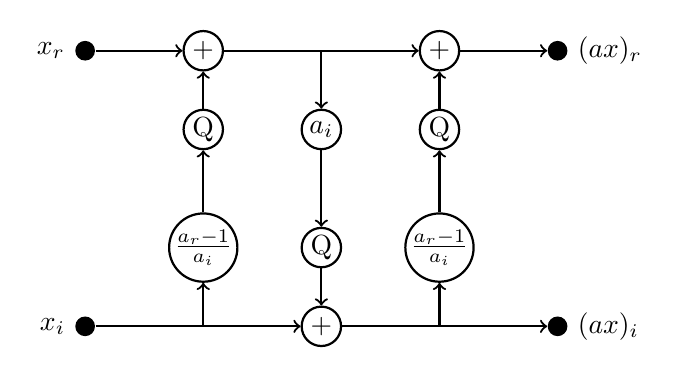
\begin{tikzpicture}[
                dot/.style = {circle, fill, inner sep = 0mm, minimum size = 2.5mm},
                op/.style = {draw, thick, circle, inner sep = 0mm, minimum size = 5mm},
                func/.style = {draw, thick, circle, inner sep = 1mm},
                arr/.style = {draw, thick, ->},
            ]
            \node (xr) [dot, label=left:$x_r$] at (0,3.5){};
            \node (xi) [dot, label=left:$x_i$] at (0,0){};
            \node (axr) [dot, label=right:$(ax)_r$] at (6,3.5){};
            \node (axi) [dot, label=right:$(ax)_i$] at (6,0){};

            \node (one) [op] at (1.5, 1) {$\frac{a_r - 1}{a_i}$};
            \node (two) [op] at (3, 2.5) {$a_i$};
            \node (three) [op] at (4.5, 1) {$\frac{a_r - 1}{a_i}$};

            \node (q1) [op] at (1.5, 2.5){Q};
            \node (q2) [op] at (3, 1){Q};
            \node (q3) [op] at (4.5, 2.5){Q};

            \node (p1) [op] at (1.5, 3.5){+};
            \node (p2) [op] at (3, 0){+};
            \node (p3) [op] at (4.5, 3.5){+};

            \path[arr] (xr) -- (p1);
            \path[arr] (p1) -- (p3);
            \path[arr] (p3) -- (axr);

            \path[arr] (xi) -- (p2);
            \path[arr] (p2) -- (axi);

            \path[arr] (1.5, 0) -- (one);
            \path[arr] (one) -- (q1);
            \path[arr] (q1) -- (p1);

            \path[arr] (3, 3.5) -- (two);
            \path[arr] (two) -- (q2);
            \path[arr] (q2) -- (p2);

            \path[arr] (4.5, 0) -- (three);
            \path[arr] (three) -- (q3);
            \path[arr] (q3) -- (p3);
        \end{tikzpicture}
        \caption{Lifting scheme with quantization.\label{fig:complexmulc}}
    \end{subfigure}
    \caption{Datapaths for complex multiplication.\label{fig:complexmul}}
\end{figure}


\subsection{Reversible convolution}
As can be seen quite clearly in the FFT datapath example (figure \ref{fig:lattice}),
merging the results of recursive steps requires a second butterfly update.
This time, we need to compute
$x_\text{new} = x + y$ and $y_\text{new} = x - y$ in-place (figure \ref{fig:conva}).
This is a reversible computation, as the original value of $y$ can be retrieved with
$y = (x_\text{new} - y_\text{new})/2$, and $x$ can be retrieved with $x = x_\text{new} - y$.
We can encode this reversibility by implementing the convolution as lifting steps,
as seen in figure \ref{fig:convb}.

\begin{figure}[h]
    \centering
    \begin{subfigure}[b]{0.496\textwidth}
        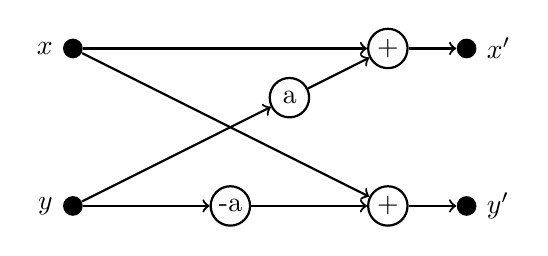
\begin{tikzpicture}[
                dot/.style = {circle, fill, inner sep = 0mm, minimum size = 2.5mm},
                op/.style = {draw, thick, circle, inner sep = 0mm, minimum size = 5mm},
                func/.style = {draw, thick, circle, inner sep = 1mm},
                arr/.style = {draw, thick, ->},
            ]
            \node (x) [dot, label=left:$x$] at (0,2){};
            \node (y) [dot, label=left:$y$] at (0,0){};
            \node (xp) [dot, label=right:$x'$] at (5,2){};
            \node (yp) [dot, label=right:$y'$] at (5,0){};

            \node (a1) [op] at (2.75, 1.375) {a};
            \node (a2) [op] at (2, 0) {-a};
            \node (p1) [op] at (4, 2) {+};
            \node (p2) [op] at (4, 0) {+};

            \path[arr] (x) -- (p1);
            \path[arr] (p1) -- (xp);
            \path[arr] (y) -- (a2);
            \path[arr] (a2) -- (p2);
            \path[arr] (p2) -- (yp);

            \path[arr] (x) -- (p2);

            \path[arr] (y) -- (a1);
            \path[arr] (a1) -- (p1);
        \end{tikzpicture}
        \caption{Butterfly structure.\label{fig:conva}}
    \end{subfigure}
    \begin{subfigure}[b]{0.496\textwidth}
        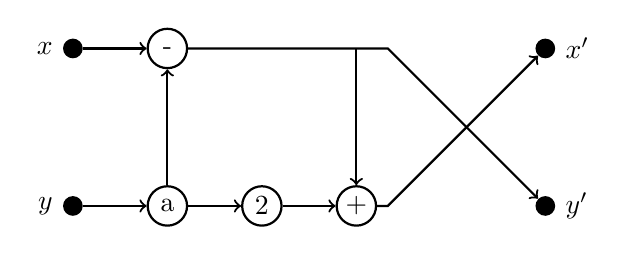
\begin{tikzpicture}[
                dot/.style = {circle, fill, inner sep = 0mm, minimum size = 2.5mm},
                op/.style = {draw, thick, circle, inner sep = 0mm, minimum size = 5mm},
                func/.style = {draw, thick, circle, inner sep = 1mm},
                arr/.style = {draw, thick, ->},
            ]
            \node (x) [dot, label=left:$x$] at (0,2){};
            \node (y) [dot, label=left:$y$] at (0,0){};
            \node (yp) [dot, label=right:$y'$] at (6,0){};
            \node (xp) [dot, label=right:$x'$] at (6,2){};

            \node (a) [op] at (1.2,0){a};
            \node (t) [op] at (2.4,0){2};
            \node (m) [op] at (1.2,2){-};
            \node (p) [op] at (3.6,0){+};

            \path[arr] (x) -- (m);
            \path[arr] (y) -- (a);
            \path[arr] (a) -- (m);
            \path[arr] (a) -- (t);
            \path[arr] (t) -- (p);
            \path[arr] (3.6,2) -- (p);

            \path[arr] (m) -- (4, 2) -- (yp);
            \path[arr] (p) -- (4, 0) -- (xp);
        \end{tikzpicture}
        \caption{Alternative lifting scheme.\label{fig:convb}}
    \end{subfigure}
    \caption{Datapaths for FFT convolution.\label{fig:conv}}
\end{figure}


This introduces a significant challenge to the reversibility of our algorithm.
This operation isn't \textit{only} implemented through lifting steps,
but requires an in-place doubling of $y$.
Integer multiplications are only injective,
as outputs must be a multiple of the factor for them to correspond to an input value.
As a result, the inverse is only partially defined, for outputs that are a factor of 2 apart.
This issue isn't covered by \cite{intfft}.
When reversing, you can divide by 2 and round off the result to get a decent result
without changing the semantics for valid outputs.
This strategy won't work in a fully reversible system however.

For our implementation,
we write a multiplication function that panics when run in reverse on uneven output.
This does have the disadvantage that our inverse FFT doesn't work on all outputs.
There may be workarounds for this issue,
but that wont be explored in the scope of this project.

\subsection{Bit resolution}
At this point,
all parts of the algorithm have been molded into reversible operations.
While the algorithm is reversible,
the output \textit{does} require more bits to represent than the input.

The offenders that produce these bits are the twiddle factor multiplications and convolutions.
It should be fairly obvious to see that convolution increases bit-depth by one,
as it effectively only performs either a subtraction or addition to the target variables.
It isn't hard to see that convolution increases the bit-depth of the complex components by 1.
For multiplication, the quantization in the lifting scheme (figure \ref{fig:complexmulc})
step removes the worst of the bit-depth increase.
That leaves three additions, each increasing the depth by one bit.
While \cite{intfft} does prove
that we can limit the increase for twiddle factor multiplication to one bit,
we settle for a bound of 3 bits.

For every recursive step of the algorithm,
each cell of our input array may be multiplied by one coefficient
and will be convoluted with another cell.
That makes for a 4 bit depth-increase per layer, and total a limit of $4 \log_2 N$ additional bits.
